%----------------------------------------------------------------------------------------
%	PACKAGES AND OTHER DOCUMENT CONFIGURATIONS
%------------------------------------------------------------------------
\documentclass[11pt]{article}
\usepackage[utf8]{inputenc} % Required for inputting international characters
\usepackage[T1]{fontenc} % Output font encoding for international characters
\usepackage{mathpazo} % Palatino font
\usepackage[czech]{babel} % Czech
\usepackage{graphicx}  % Graphics
%\usepackage[amsmath]

\begin{document}

%----------------------------------------------------------------------------------------
%	TITLE PAGE
%----------------------------------------------------------------------------------------

\begin{titlepage} % Suppresses displaying the page number on the title page and the subsequent page counts as page 1
	\newcommand{\HRule}{\rule{\linewidth}{0.5mm}} % Defines a new command for horizontal lines, change thickness here
	
	\center % Centre everything on the page
	
	%------------------------------------------------
	%	Headings
	%------------------------------------------------
	
	\textsc{\LARGE České vysoké učení technické v Praze}\\[1.5cm] % Main heading such as the name of your university/college
	
	\textsc{\Large Algoritmy digitální kartografie a GIS}\\[0.5cm] % Major heading such as course name
	
	\textsc{\large Katedra geomatiky}\\[0.5cm] % Minor heading such as course title
	
	%------------------------------------------------
	%	Title
	%------------------------------------------------
	
	\HRule\\[0.4cm]
	
	{\huge\bfseries Úloha č. 3: Digitální model terénu}\\[0.4cm] % Title of your document
	
	\HRule\\[1.5cm]
	
	%------------------------------------------------
	%	Author(s)
	%------------------------------------------------
	
	

	
	% If you don't want a supervisor, uncomment the two lines below and comment the code above
	Monika \textsc{Křížová} % Your name
	
	Marek \textsc{Hoffmann}
	
	%------------------------------------------------
	%	Date
	%------------------------------------------------
	
	\vfill\vfill\vfill % Position the date 3/4 down the remaining page
	
	{\large 4.12.2021} % Date, change the \today to a set date if you want to be precise
	
	%------------------------------------------------
	%	Logo
	%------------------------------------------------
	
	%\vfill\vfill
	%\includegraphics[width=0.2\textwidth]{placeholder.jpg}\\[1cm] % Include a department/university logo - this will require the graphicx package
	 
	%----------------------------------------------------------------------------------------
	
	\vfill % Push the date up 1/4 of the remaining page
	
\end{titlepage}

%----------------------------------------------------------------------------------------


%----------------------------------------------------------------------------------------
%	TABLE OF CONTENT
%----------------------------------------------------------------------------------------

\tableofcontents
%\thispagestyle{empty}

\clearpage

%----------------------------------------------------------------------------------------
%	ZADÁNÍ
%----------------------------------------------------------------------------------------

\section{Zadání}
Navrhněte aplikaci s grafickým rozhraním, která nad množinou bodů vytvoří polyedrický digitální model terénu.

Jako vstupní data využijte existující data o alespoň 300 bodech. Nad nimi vytvořte Delaunayovu triangulaci metodou inkrementální konstrukce. Triangulaci využijte pro výpočet a vykreslení vrstevnic. Výslednou triangulaci doplňte o vhodnou vizualizaci sklonu jednotlivých trojúhelníků a jejich expozici. 

%----------------------------------------------------------------------------------------
%	BONUSOVÉ ÚLOHY
%----------------------------------------------------------------------------------------

\section{Údaje o bonusových úlohách}
Zpracovány byly celkem 3 bonusové úlohy ze 7 zadaných.

\begin{itemize}
	\item Triangulace nekonvexní oblasti zadané polygonem +5b
	\item Výběr barevných stupnic při vizualizaci sklonu a expozice. +3b
	\item Automatický popis vrstevnic respektující kartografické zásady +10b - z části
	
\end{itemize}

%----------------------------------------------------------------------------------------
%	POPIS PROBLÉMU
%----------------------------------------------------------------------------------------

\section{Popis problému}
Triangulace je jednou ze základních výpočetních úloh nejen v oblasti digitální kartografie. Kromě tvorby DMT své uplatnění najde i při tvorbě jakékoliv vizualizace prostorových dat ve formě 3D modelů. Dále lze triangulaci využít při detekci otisku prstů či např. modelování přírodních jevů.
 
\subsection{Formulace problému}

Mějme množinu bodů $P$. Triangulací se rozumí převod množiny bodů na trojúhelnikovou síť $m$ trojúhelníků $t$ tak, aby platilo:

\begin{itemize}
	\item Libovolné 2 trojúhelníky mají společnou nejvýše jednu hranu.
	\item Sjednocení trojúhelníků je souvislá množina.
	\item Uvnitř žádného trojúhelníku neleží žádný další bod z $P$.	
\end{itemize}

Triangulace by měla tvořit pravidelné trojúhelníky blížící se trojúhelníkům rovnostranným a všechny trojúhelníky by se v každém bodě měly co nejlépe přimykat terénu. 

%----------------------------------------------------------------------------------------
%	POPIS ALGORITMŮ
%----------------------------------------------------------------------------------------

\section{Popisy algoritmů}
\subsection{Delaunayova triangulace}

Existuje několik druhů triangulace. Nejpoužívanějsí je však Delaunayova triangulace, která svými kritérii zajišťuje jednoznačnost, spolehlivé výslekdy a má optimální časovou složitost. Tyto požadavky jsou následující:

\begin{itemize}
\item Uvnitř kružnice $k$ opsanému libovolnému trojúhelníku $t_{j}$ neleží žádný jiný bod množiny $P$.
\item $DT$ maximalizuje minimální úhel v každém $t_{j}$, ale neminimalizuje maximální úhel v $t_{j}$. 
\item $DT$ je lokálně i globální optimální vůči kritériu minimálního úhlu.
\item $DT$ je jednoznačná, pokud žádné 4 body neleží na kružnici.

\end{itemize}

\subsubsection{Inkrementální konstrukce}
Existuje několik metod konstrukce Delaunayho triangulace. V této úloze však byla implementována metoda inkrementální konstrukce, která je založena na postupném přidávání bodů do již vytvořené triangulace.

Pro konstrukci je používána datová struktura AEL (Active Edge List), která obsahuje hrany $e$, ke kterým hledáme Delaunayovský bod minimalizující poloměr kružnice mezi Delaunayovskou hranou a hledaným bodem. Delaunayovská hrana je orientovaná a bod hledáme pouze vlevo od ní.

 \paragraph{Popis Algoritmu}
 
 \begin{enumerate}
 \item Nalezení bodu $q$ s nejmenší x-ovou souřadnicí 
 $$ q = min(x_i) $$ 
 \item Nalezení nejbližšího bodu k počátečnímu bodu 
 $$ ||p_1 - q||_2 = min  $$
 \item Vytvoření první hrany 
 $$ e = (q, p_1) $$
 \item Hledání Delaunayho bodu 
 $$ \underline{p} = argmin_{\forall p_i \in \sigma_L (e)} r'(k_i); k_i = (a, b, p_i); e = (a, b)$$
 \item Při neexistenci Delaunayho bodu změna orientace hrany a opakování předchozího kroku
 $$ \not\exists \underline{p} : e \leftarrow (p_1, q);$$
 
 \item Vytvoření zbývajících hran trojúhelníka 
 $$ e_2 = (p_1,  \underline{p}); e_3 = ( \underline{p} , q) $$
 \item Přidání hran do AEL 
 $$ AEL \leftarrow e; AEL \leftarrow e_2; AEL \leftarrow e_3  $$  
 \item Přidání hran do DT  
 $$ DT \leftarrow e; DT \leftarrow e_2; DT \leftarrow e_3  $$
 \item Dokud není vektor AEL prázdný: 
 
		Změna orientace první hrany z AEL
	$$ e = (p_1, q) $$
		Hledání Delaunayho bodu k e 
	$$ \underline{p} = argmin_{\forall p_i \in \sigma_L (e)} r'(k_i); k_i = (a, b, p_i); e = (a, b)$$ 
		Pokud bod existuje 
	$$ if \exists  \underline{p}$$
		Tvorba zbývajících hran trojúhelníku 
		$$ e_2 = (p_2,  \underline{p}); e_3 = ( \underline{p} , q) $$
		Přidání hran do DT 
		$$ DT \leftarrow e; DT \leftarrow e_2; DT \leftarrow e_3  $$
		Přidání hrany do AEL, pokud již neexistuje s opačnou orientací.
		$$AEL if \not\exists \leftarrow e_2; AEL \leftarrow e_3  $$ 
 \end{enumerate}


\subsection{Konstrukce vrstevnic lineární interpolací}
Vrstevnice je křivka, která spojuje body se stejnou nadmořskou výškou. Zpravidla bývají vrstevnice vykreslovány s pravidelným intervalem.

Vrstevnice dělíme na základní a hlavní. Základní vrstevnice tvořené s pravidelným základním intervalem bývají vyznačeny tenkou, nepřerušovanou linií a jsou uzavřené. Hlavní vrstevnice je každá pátá základní vrstevnice. V mapách bývá značena tlustou, nepřerušovanou, uzavřenou linií a bývají doplněny popisem.

Dále existují vrstevnice doplňkové, které doplňují základní vrstevnice v těch místech, kde dostatečně nevystihují zejména sklonitý terén, a vrstevnice pomocné, které se používají pro místa s nestálým reliéfem jako např. v oblastech povrchové těžby. Doplňkové ani pomocné vrstevnice nebyly v této aplikaci implementovány.

\subsubsection{Lineární interpolace}
Lineární interpolace předpokládá:
\begin{enumerate}
\item Spád terénu mezi dvěma body, mezi kterými provádíme interpolaci, je konstantní.
\item Rozestup vrstevnic mezi dvěma body je konstantní.
\end{enumerate}

Na vstupu máme trojúhelník $t$ a vodorovnou rovinu $\rho$ o výšce $h$. Lineární interpolace je založena na analytické geometrii. Hledáme tedy průsečnici roviny $T$ určené trojúhelníkem $t$ a vodorovnou rovinou. Tento výpočet provedeme nad každým trojúhelníkem $t$

\subsubsection{Algoritmus}

\begin{enumerate}
\item Nalezení průsečíků všech horizontálních rovin s jednotlivými hranami.

Varianty vzájemné polohy $\rho$ a $T$:
	\begin{enumerate}
		\item Nemají žádný společný bod - neřešíme.
		\item Průsečnice tvoří jeden bod - neřešíme.
		\item Průsečnice je úsečka:
		\begin{itemize}
		\item Hrana leží v rovině $\rho$ - vrstevnice je přímo v hraně.
		\item Průsečnice roviny s trojúhelníkem vytvářející nové průsečíky mezi vrcholy trojúhelníku - vrstevnice je vykreslena mezi body vypočtenými následujícími rovnicemi:
		$$  x = \frac{(x_2 - x_1)}{(z_2 - z_1)} (z - z_1) + x_1 $$ 
		
$$  y = \frac{(y_2 - y_1)}{(z_2 - z_1)} (z - z_1) + y_1 $$ 
		\end{itemize}
		\item Všechny hrany trojúhelníku leží v rovině $\rho$ - neřešíme.	
	\end{enumerate}

\end{enumerate}
 
\subsection{Algoritmus výpočtu sklonu trojúhelníku}
Sklon představuje jednu z analytických úloh realizovaných nad DMT. Určuje, zdali terén stoupá, klesá nebo je rovinný.

Sklon každého trojúhelníku se vypočte následujícím způsobem.

$$  u = (u_x, u_y, u_z)
$$

$$  v = (v_x, v_y, v_z)
$$

$$ n = \vec{u}\times \vec{v} = (n_x, n_y, n_z)$$
  
$$ \varphi = arccos \frac{n_z}{|n|} $$ 



\subsection{Algoritmus výpočtu expozice trojúhelníku}
Expozice představuje orientaci terénu vzhledem ke Slunci.

Orientace v bodě je definován jako azimut průmětu normálového vektoru roviny trojúhelníku do roviny x,y.


$$  u = (u_x, u_y, u_z)
$$

$$  v = (v_x, v_y, v_z)
$$

$$ n_t = \vec{u}\times \vec{v} = (n_x, n_y, n_z)$$

$$ A =atan2( \frac{n_x}{n_y}) $$

%----------------------------------------------------------------------------------------
%	PROBLEMATICKÉ SITUACE
%----------------------------------------------------------------------------------------
\section{Problematické situace}

\subsection{idk}


\subsection{idk}

\clearpage



%----------------------------------------------------------------------------------------
%	VSTUPNÍ DATA
%----------------------------------------------------------------------------------------


\section{Vstupní data}

Polygonová mapa se do projektu nahrává z textového souboru, který musí splňovat specifický formát, bez něhož nebude zajištěno správné načítání dat.  

Vrcholy polygonů jsou načítány postupně řádek po řádku, přičemž musí v nahrávaném souboru platit následující pravidla:    

\begin{itemize}
\item každý vrchol polygonu je definován na jednotlivém řádku,
\item na řádku je pořadí proměnných id >> x >> y   ,  hodnoty jsou od sebe odděleny  jednou mezerou,
\item id je identifikátor jednotlivých vrcholů polygonu, x a y jsou souřadnice vrcholů polygonu,    
\item nový polygon má vždy hodnotu id prvního vrcholu rovnu 1, od této hodnoty  se  postupně načítají body, a  to až do okamžiku,  kdy program dojde  k dalšímu identifikátoru s označením 1.   
\end{itemize}

\begin{figure}[htbh]
	\centering
	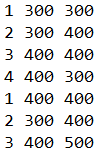
\includegraphics[scale=1]{images/vstup.png} 
	\caption{Špagetový model vstupního souboru}
	\label{fig:vstup.}
\end{figure} 

Souřadnice bodu $q$ jsou získávány interaktivně odečtením souřadnic kurzoru myši.   

\clearpage

%----------------------------------------------------------------------------------------
%	VÝSTUPNÍ DATA
%----------------------------------------------------------------------------------------

\section{Výstupní data}

Po načtení souboru s polygonovou mapou, přidání bodu $q$ a stisknutí tlačítka Analyze se v místě vyznačeném na obrázku \ref{fig:app_analyze} vytiskne výsledek analýzy polohy bodu. 

\begin{figure}[htbh]
	\centering
	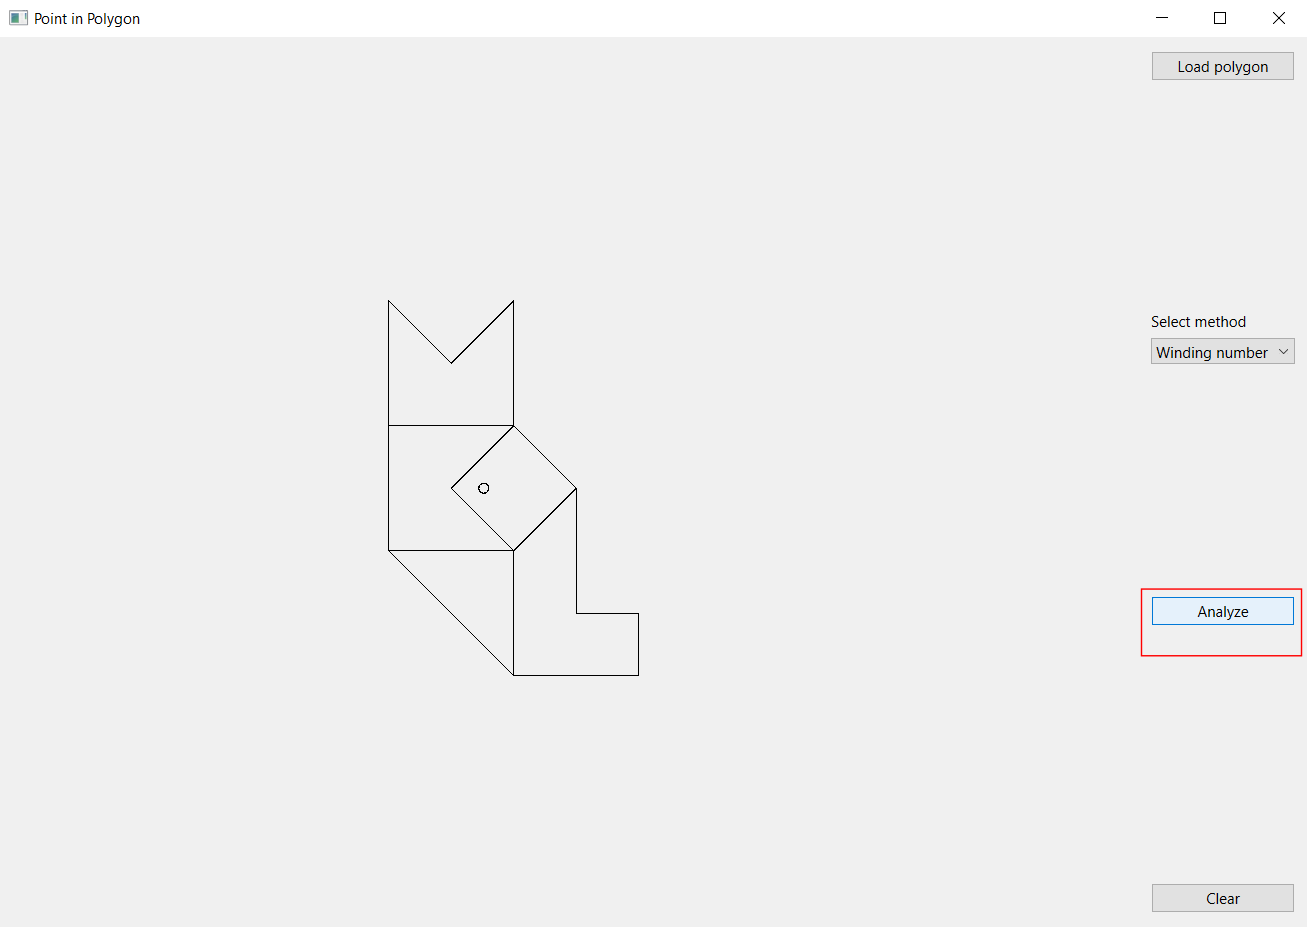
\includegraphics[scale=0.4]{images/aplikace_klik_analyze.png} 
	\caption{Aplikace s načteným polygonem}
	\label{fig:app_analyze}
\end{figure} 

Výsledek dotazu může mít 3 různé hodnoty:

\begin{itemize}
\item je-li bod mimo polygonovou mapu, vypíše se zpráva „Outside“,
\item je-li bod uvnitř polygonu, vypíše se zpráva „Inside“ a polygon obsahující zadaný bod se graficky zvýrazní,
\item je-li bod na hranici polygonu, vypíše se „Point is on the line“ a graficky se zvýrazní polygon, na jehož linii bod leží.      
\end{itemize}
\begin{figure}[htbh]
	\centering
	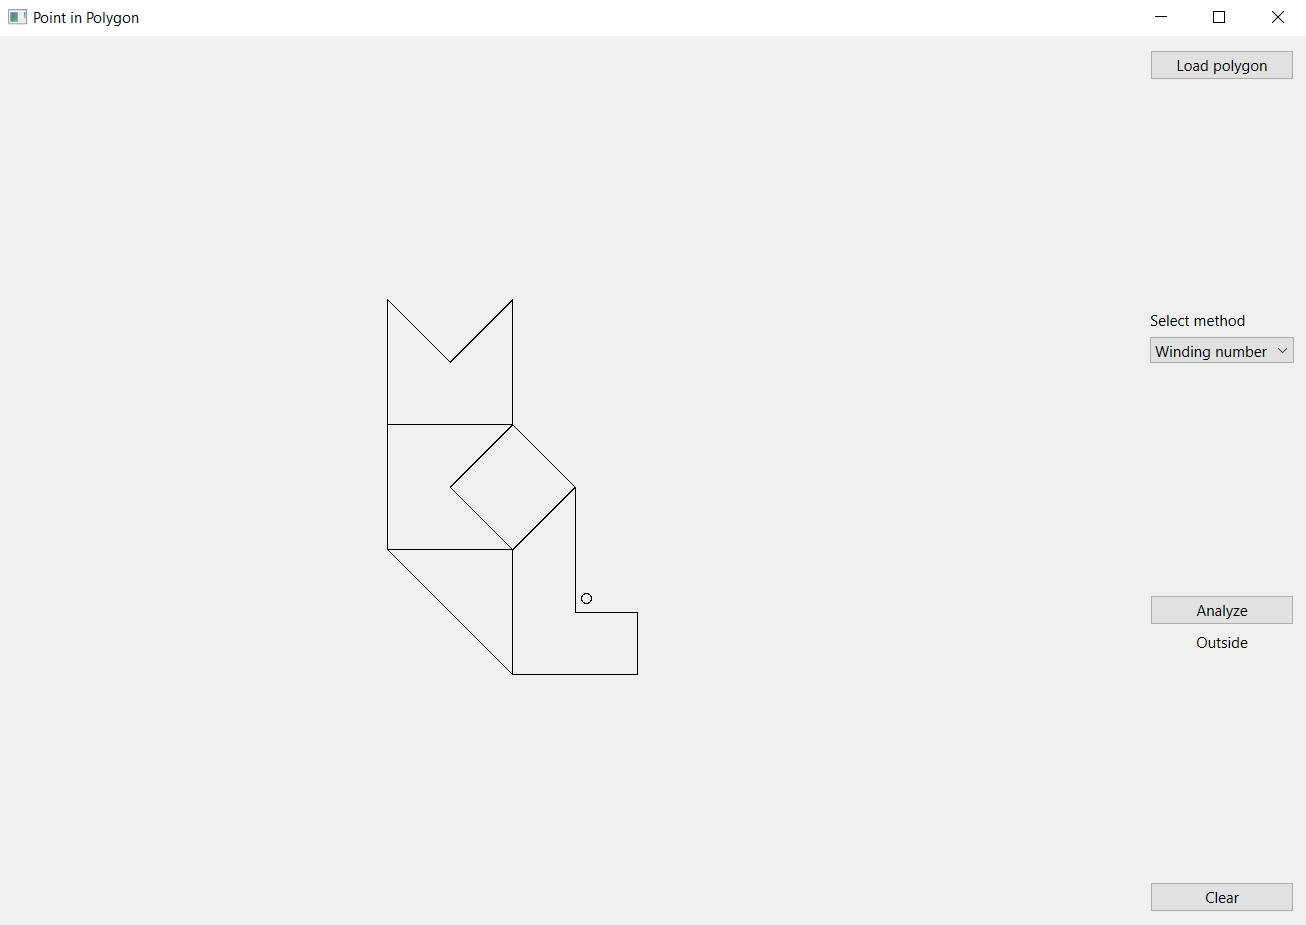
\includegraphics[scale=0.4]{images/aplikace_analyze_outside.png} 
	\caption{Bod vně polygonu}
	\label{fig:app_outside}
\end{figure} 
\begin{figure}[htbh]
	\centering
	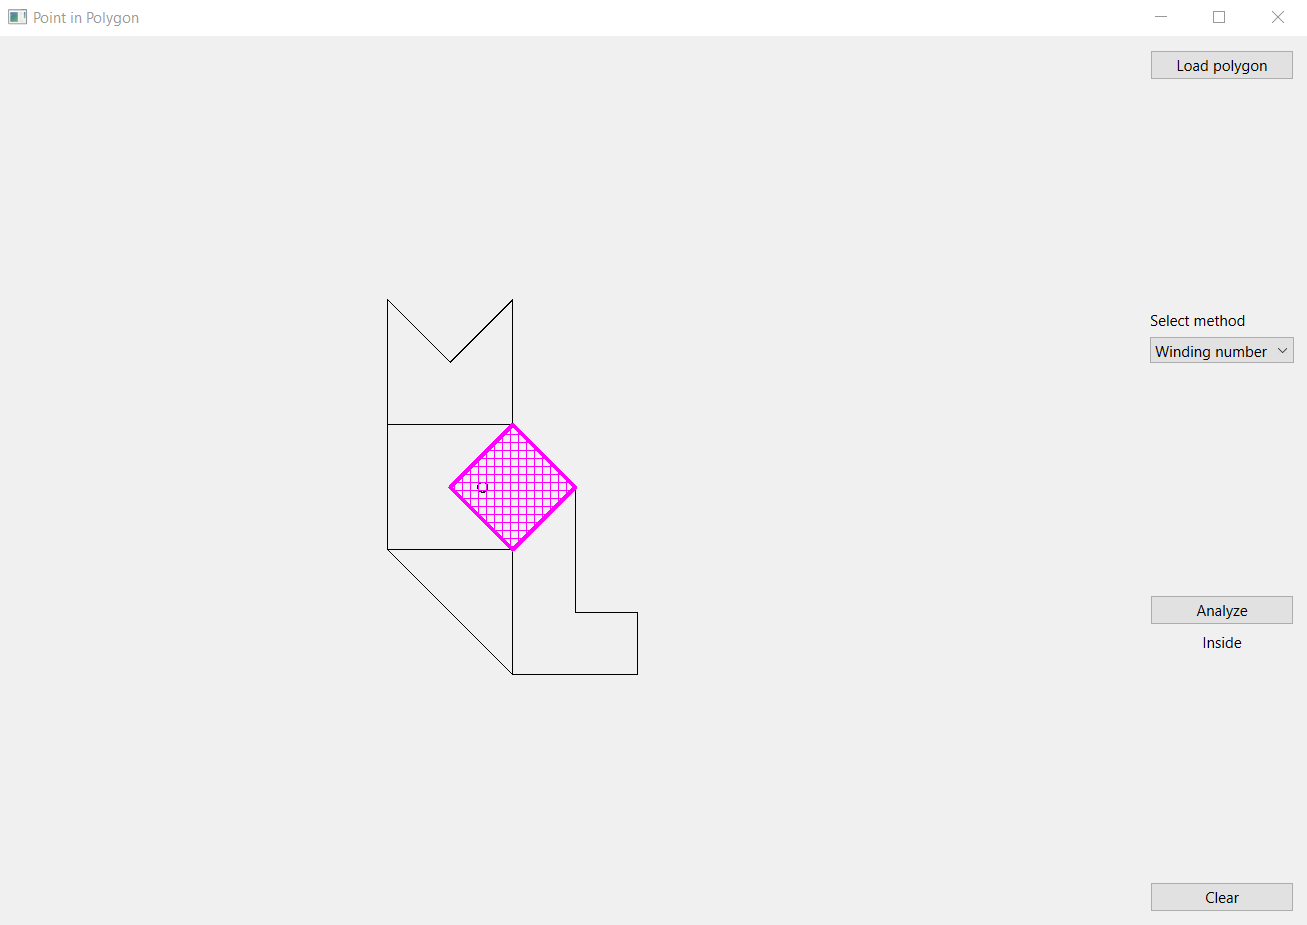
\includegraphics[scale=0.4]{images/aplikace_analyze_inside.png} 
	\caption{Bod uvnitř polygonu}
	\label{fig:app_inside}
\end{figure} 

\clearpage

\section{Printscreen vytvořené aplikace}
\begin{figure}[htbh]
	\centering
	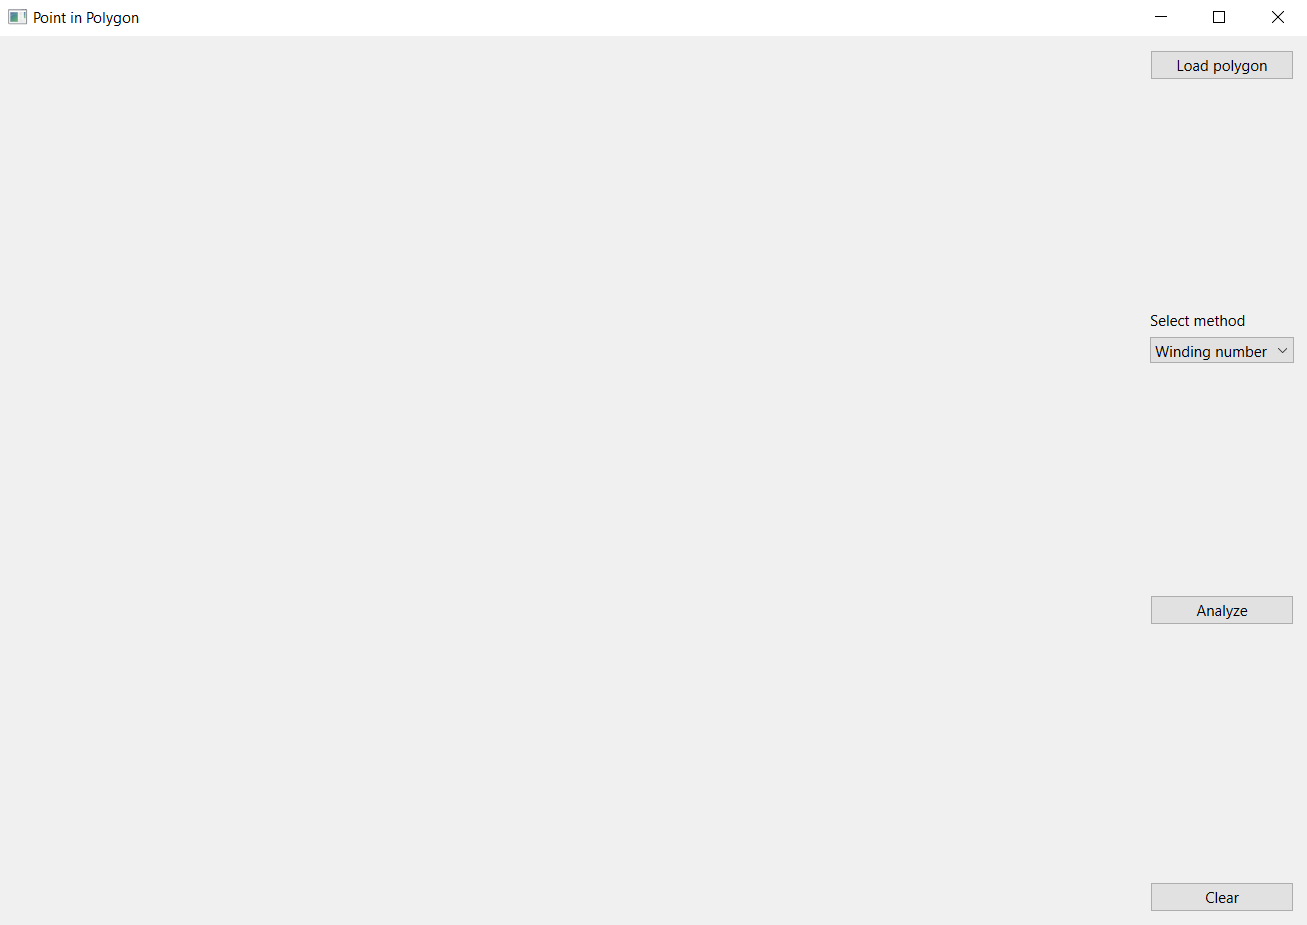
\includegraphics[scale=0.4]{images/aplikace_uvodni_okno.png} 
	\caption{Úvodní okno aplikace}
	\label{fig:uvodni_okno}
\end{figure} 

%----------------------------------------------------------------------------------------
%	DOKUMENTACE
%----------------------------------------------------------------------------------------

\section{Dokumentace}
Kód zahrnuje 3 třídy – Draw, Algorithms a Widget, které budou následně detailněji popsány.      

\subsection{Třída Algorithms}
Třída Algorithms obsahuje 4 funkce :  

\begin{itemize}
\item int getPointLinePosition(QPoint \&a, QPoint \&p1, QPoint \&p2);
\item double get2LinesAngle(QPoint \&p1, QPoint \&p2, QPoint \&p3, QPoint \&p4);
\item int getPositionWinding(QPoint \&q, std::vector<QPoint> \&pol);
\item int getPositionRayCrossing(QPoint \&q, std::vector<QPoint> \&pol);
\end{itemize}

\paragraph{int getPointLinePosition(QPoint \&a, QPoint \&p1, QPoint \&p2);}\mbox{}\\
Analyzuje vzájemnou polohu mezi bodem a linií polygonu, resp. v jaké polorovině vůči linii se bod nachází. Vstupními argumenty funkce jsou souřadnice určovaného bodu (jako QPoint) a souřadnice 2 bodů určujících polohu linie (vrcholy polygonu taktéž jako QPoint). Funkce vrací vždy hodnotu 1, 0 nebo -1 dle následujících pravidel:

\begin{itemize}
\item 0 v případě, že bod leží v pravé polorovině,
\item 1 v případě, že  bod leží v levé polorovině,
\item -1 v případě, že bod leží na linii.
\end{itemize}

\paragraph{double get2LinesAngle(QPoint \&p1, QPoint \&p2, QPoint \&p3, QPoint \&p4);}\mbox{}\\
Počítá úhel mezi dvěma liniemi pomocí vztahu \ref{WN:omega_i}. Vstupními argumenty jsou body určující linie, tzn. vrcholy polygonu. Návratovou hodnotou funkce je double – desetinné číslo s velikostí úhlu mezi těmito přímkami.  

\paragraph{int getPositionWinding(QPoint \&q, std::vector<QPoint> \&pol);}\mbox{}\\
Funkce analyzuje polohu bodu metodou Winding Number, jež byla podrobně vysvětlena v kapitole 3.  Vstupními argumenty jsou souřadnice bodu $q$ (jako QPoint) a vektor vrcholů polygonu (vektor naplněný prvky QPoint). Funkce vrací integer, jež může nabývat 3 hodnot:

\begin{itemize}
\item 1, leží-li analyzovaný bod uvnitř polygonu
\item -1 leží-li na linii polygonu 
\item a 0, leží-li mimo kontrolovaný polygon.
\end{itemize}

\paragraph{int getPositionRayCrossing(QPoint \&q, std::vector<QPoint> \&pol);}\mbox{}\\
Funkce analyzuje polohu bodu metodou Ray Crossing, jež byla podrobně vysvětlena v kapitole 3. vstupními argumenty jsou souřadnice bodu $q$ (jako QPoint) a vektor vrcholů polygonu (vektor naplněný prvky QPoint). Funkce vrací, stejně jako funkce předchozí, celé číslo, jež může nabývat následujících hodnot:

\begin{itemize}
\item 1, pokud leží analyzovaný bod uvnitř polygonu
\item a 0, leží-li mimo kontrolovaný polygon.
\end{itemize}

Ošetření případu, kdy bod leží na linii nebylo do kódu implementováno, funkce tedy nevrací  hodnotu -1, leží-li bod na linii.

\subsection{Třída Draw}
Třída Draw obsahuje následující funkce, které budou dále podrobně popsány:

\begin{itemize}
\item void paintEvent(QPaintEvent *event);
\item void mousePressEvent(QMouseEvent *event);
\item void clear();
\item QPoint getPoint(){return q;}
\item std::vector<QPolygon> getPolygon()\{return polygons;\}
\item void fillPolygon(int result);
\item void loadData(QString \&file\_name);
\end{itemize}

a následující proměnné:

\begin{itemize}
\item std::vector<QPolygon> polygons;  
\item QPoint q; - analyzovaný bod
\item int highlighted\_polygon=-99; - id polygonu, který obsahuje analyzovaný bod   
\end{itemize}

\paragraph{•	void paintEvent(QPaintEvent *event);}\mbox{}\\
Funkce nastavuje grafické atributy vykreslovaných objektů a kreslí na plátno vyhodnocovaný bod a zadané polygony a znázorňuje polygon incidující s bodem. 

\paragraph{void mousePressEvent(QMouseEvent *event);}\mbox{}\\
Metoda získává souřadnice myši a ukládá je do proměnné QPoint q, tedy jako souřadnice analyzovaného bodu $q$.

\paragraph{void clear();}\mbox{}\\
Funkce smaže veškeré objekty, jež jsou vykresleny na canvasu, funkce nemá vstupní argumenty. 

\paragraph{QPoint getPoint()\{return q;\}}\mbox{}\\
Funkce vrací souřadnice bodu $q$, návratový typ funkce je QPoint, funkce nemá vstupní argumenty.

\paragraph{std::vector<QPolygon> getPolygon()\{return polygons;\}}\mbox{}\\
Funkce vrací vektor polygonů načtených z textového souboru – návratový typ je std::vector<QPolygon>, funkce nemá vstupní argumenty.

\paragraph{void fillPolygon(int result);}\mbox{}\\
Funkce ukládá identifikátor polygonu obsahujícího analyzovaný bod, pomocí identifikátoru se tento polygon následně ve funkci paintEvent() zvýrazní. Vstupním argumentem je int result, jež stanovuje polohu bodu vůči linii (má hodnoty 0,1,-1,dle definice výše). 

\paragraph{void loadData(QString \&file\_name);}\mbox{}\\
Funkce načítá data z textového souboru a ukládá je do vektoru QPolygon. Vstupní argumentem je cesta k souboru, jejž chceme načíst do aplikace.   

\subsection{Třída Widget}
Třída Widget obsahuje 3 metody:

\begin{itemize}
\item void on\_pushButtonClear\_clicked();
\item void on\_pushButtonAnalyze\_clicked();
\item void on\_pushButtonLoad\_clicked();
\end{itemize}

\paragraph{ void on\_pushButtonClear\_clicked();}\mbox{}\\
Funkce se volá při stisknutí tlačítka Clear, volá funkci clear(), jež je definovaná v třídě Draw.

\paragraph{ void on\_pushButtonAnalyze\_clicked();}\mbox{}\\
Funkce se volá při stisknutí tlačítka Analyze. Ve funkci nejprve dojde k uložení jednotlivých polygonů do vektoru vrcholů polygonu, následně je zavolána funkce getPositionRayCrossing ze třídy Algorithms nebo getPositionWinding dle výběru v comboboxu.

\paragraph{void on\_pushButtonLoad\_clicked();}\mbox{}\\
Funkce slouží k inicializaci načítání souboru, spustí se po stisknutí tlačítka Load, čímž zobrazí dialog pro výběr souboru obsahujícího data, jež mají být načtena do aplikace. Po výběru souboru se zavolá funkce loadData ze třídy Draw, která přečte data ze souboru a uloží je do proměnné.

%----------------------------------------------------------------------------------------
%	ZÁVĚR
%----------------------------------------------------------------------------------------

\section{Závěr}
Vytvořená aplikace vizualizuje polygonovou mapu uloženou ve výše popsaném formátu, po přidání bodu taktéž analyzuje polohu tohoto bodu vůči jednotlivým polygonům mapy. Po analýze bodu se vypíše výsledek – tedy zda bod leží uvnitř nebo vně polygonové mapy, v případě umístění bodu uvnitř polygonu se polygon obsahující tento bod graficky zvýrazní.\\

 V aplikaci jsou pro vyhodnocení polohy bodu implementovány 2 algoritmy – Winding number a Ray Crossing, mezi nimiž je možné přepínat pomocí comboboxu umístěném v pravé části okna. Princip fungování obou algoritmů je popsán v kapitole 3. \\

Možné zlepšení kódu programu by bylo v řešení singularit polohy bodu $q$, tedy případu, kdy bod $q$ leží na vrcholu jednoho či více polygonů a dále přidání analýzy případu, kdy bod $q$ leží na linii polygonu pomocí Ray Crossing algoritmu. Dalším možným krokem pro zlepšení funkčnosti by mohlo být přidání bodu $q$ pomocí vepsání souřadnic, nikoliv pouze odečtením polohy myši.

\end{document}
